\documentclass{article}
\usepackage[normalem]{ulem}
\usepackage{setspace}
\usepackage{graphicx}

\begin{document}

\title{Addendum: Mathematics of Rendering in Stereoscopic Display Space}

\date{}
\author{Edward Zhang}
\maketitle
%\doublespacing
\onehalfspace
\thispagestyle{empty}

\begin{abstract}
This document shows the derivation of how to use Nvidia 3D Vision Automatic to render at a particular point in the 3D display space.
\end{abstract}
\section{Formulation}
We let $P = (x_p,y_p,z_p)$ be the coordinates in real-world space that we want to render a point at, relative to an origin at the center of the screen. The positive $x$-axis is to the viewer's right, the positive $y$-axis is upwards along the screen, and the positive $z$-axis is perpendicular to the screen towards the viewer.

We let $x,y,z$ be the point in screen-space that produces, when 3D Vision Automatic is active, a point that appears stereoscopically at $(x_p,y_p,z_p)$.

Let $H = (x_H,y_H,z_H)$ be the coordinates of the point halfway between the left eye and right eye (the center of the head), $R$ be the size of a pixel, and $E$ be the distance from either eye to $H$ (i.e. half the eye separation). $s,c$ are the eye separation and depth offset used in 3D vision automatic. 

\section{Derivation of $x$}
Using similar triangles, we first determine the points in real-world space on the monitor that project to the appropriate point in the display space. Let $x_R, x_L$ be the $x$-coordinates of the projection of the point $P$ onto the monitor for the right and left eyes, respectively. In Figure~\ref{fig:diag}, the vertical dimensions of the triangles are fairly straightforward: $z_H$ and $z_H - z_P$. The horizontal dimensions bear a little more thought. We measure the bases of the triangles from the eye position instead of from the origin, so the two dimensions are $x_P, x_L$ offset by $\pm E - x_H$. Although the diagram is drawn in a particular configuration, the analysis holds for the case where the $x_P < x_H$.  

\begin{figure}
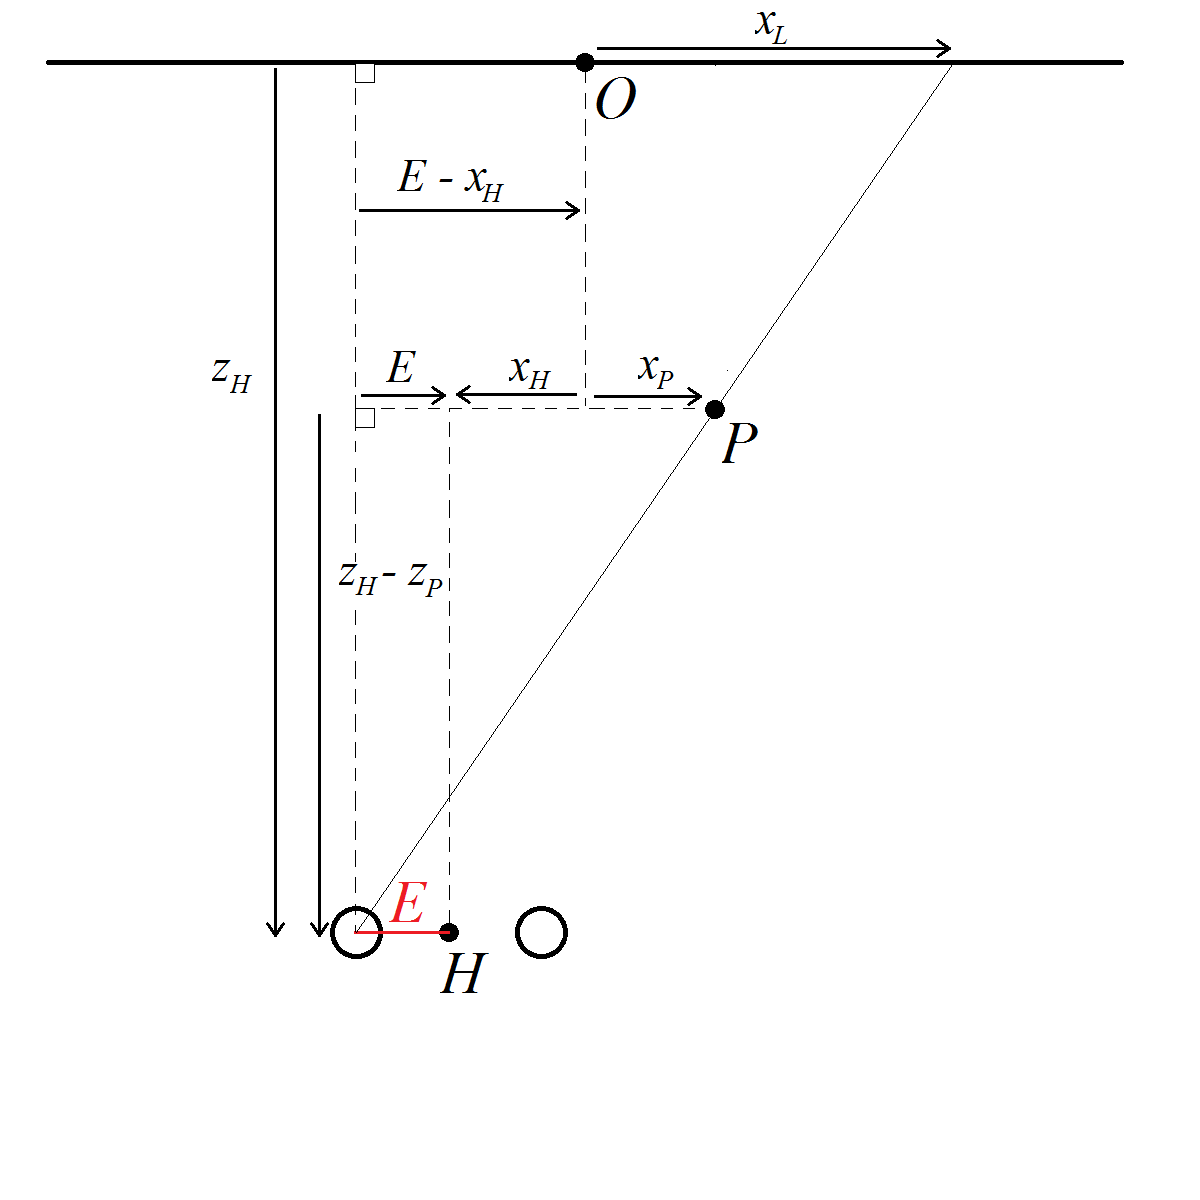
\includegraphics[width=\textwidth]{diagram.png}
\caption{Derivation of $x_L$ from similar triangles}
\label{fig:diag}
\end{figure}

Thus, we have 

$$x_R = \frac{z_H(x_p - E - x_H)}{z_H - z_p} + E + x_H = \frac{z_hx_p + z_p(-E - x_H)}{z_H - z_p}$$
$$x_L = \frac{z_H(x_p + E - x_H)}{z_H - z_p} - E + x_H = \frac{z_hx_p + z_p(E - x_H)}{z_H - z_p}$$

The midpoint of these two points, or more simply the projection from $H$ to $P$ onto the monitor, is then 
$$x_M = \frac{z_Hx_p - z_px_H}{z_H - z_p}$$

Converting this coordinate into screen-space, we determine that
$$x = \frac{z_Hx_p - z_px_H}{R(z_H - z_p)}$$

Note that determining $x_L, x_R$ is not strictly necessary to determine $x$, but will be useful in determining $z$.

\section{Derivation of $z$}
Given that 3D Vision Automatic has placed the virtual eye-space $z$-coordinate in the $w$ coordinate of the vertex when rendering, we determine that the horizontal offset of each copy of the rendered point will appear 
$s(z-c)$ away from the given $x$ coordinate. Note that, since this happens in the pixel shader, we are already operating in clip-space (i.e. the same space as our desired $x,y,z$). We then take the distance between $x_M$ and $x_R$
and set that equal to $Rs(z-c)$.
x
$$Rs(z-c) = \frac{z_Hx_p - z_px_H}{z_H - z_p} - \frac{z_Hx_p + z_p(E - x_H)}{z_H - z_p}$$
$$Rs(z-c) = \frac{z_pE}{z_H - z_p}$$

For convenience, we can set $s = E/R, c = 0$, to cancel out some terms

$$z = \frac{z_p}{z_H - z_p}$$

\section{Derivation of $y$}
The derivation of $y$ is analogous to the derivation of $x$, and is omitted for brevity.
$$y = \frac{z_Hy_p - z_py_H}{R(z_H - z_p)}$$

\section{Further work}
This addresses the idealized setting in which the head is parallel to the screen plane. It obviously does not handle the case in which the head is turned on its $y$-axis. We would also like to determine the bounds of
the viewable space for the average user, where the convergence-accomodation mismatch is too high. We would also like to determine optimal positioning of the user relative to the screen to maximize the interaction space, such that
the space within comfortable arms reach is as large as possible. Finally, we'd like to study the ranges in which small head movements have minimal effects on the apparent locations of objects.
\end{document}
